\chapter{基于检索知识冲突消解的幻觉检测方法}\label{chp:chapter4}

% 第二项研究内容针对现有RAG幻觉检测方法对外部检索知识信号利用不充分的问题，本文拟从大语言模型内部表征中的知识冲突与消解的角度出发，研究一种\emph{基于检索知识冲突消解的幻觉检测方法}。其具体贡献如下：

% \begin{itemize}
%     \item 提出一种基于检索知识冲突消解的RAG幻觉检测方法SKID（Sparse Knowledge Inconsistency Detector）。针对现有方法对外部检索知识信号利用不充分的问题，提出在SAE高维度参数空间对外部知识和内部知识进行明确定义和消解，从而构建更准确、稳定、符合设定的RAG幻觉检测信号。
%     \item 通过引入可解释的稀疏特征表征，进一步提升RAG幻觉检测方法的可解释性，使得检测不仅能够准确反映生成内容与外部知识之间的冲突程度，还能够以清晰的自然语言表达的方式解释“模型为何被判定为产生了幻觉”，从而增强方法在实际应用中的易用性和用户信任度。
%     \item 在多个RAG数据集上进行系统性评估，并针对超参数、算法变体进行多种消融实验，验证所提出方法在准确检测RAG幻觉、刻画内外知识冲突以及提升检测可解释性方面的有效性。与现有RAG幻觉检测和幻觉检测方法进行对比分析，展示其在提升检测性能和可解释性方面的优势。
% \end{itemize}

检索增强生成（Retrieval-Augmented Generation，RAG）通过引入外部检索文档，为大语言模型生成过程提供额外知识支撑，在一定程度上缓解了封闭参数知识带来的事实性错误问题。然而，RAG并未从根本上消除幻觉现象。当检索内容与模型内部参数知识存在偏差、冲突或对齐不充分时，模型仍可能生成与检索证据不一致、与事实不符甚至凭空编造的内容。现有RAG幻觉检测方法虽然已经关注到检索文档在判别中的作用，但总体上仍存在两类主要问题：其一是\emph{对外部检索知识信号的利用仍不充分}，难以对“模型内部知识—外部检索知识”之间的冲突关系进行简洁而有效的刻画；同时，许多方法给出的检测分数缺乏清晰的语义-幻觉对应关系，导致其\emph{可解释性不足}，难以回答“模型为何被判定为产生幻觉”这一关键问题。

针对上述不足，本章提出一种基于检索知识冲突消解的RAG幻觉检测方法SKID（Sparse Knowledge Inconsistency Detector）。该方法从大语言模型内部表征出发，借助稀疏自编码器（Sparse Autoencoder，SAE）将生成过程中的隐状态映射为具有语义可解释性的稀疏特征，并通过互信息筛选得到与正确性最相关的判别维度；在此基础上，进一步结合检索文档对生成内容进行过滤，重点关注未被外部知识支持的生成片段，从而更直接地刻画模型内部知识与外部检索知识之间的冲突程度。随后，SKID利用可解释的广义加性模型对上述冲突信号进行建模，实现对RAG幻觉的有效检测。该方法不仅强化了对外部检索知识信号的直接利用，而且能够以自然语言形式揭示关键稀疏特征对判别结果的贡献，从而兼顾检测性能与结果可解释性，为RAG场景下的幻觉检测提供了一种新的技术路径。

\section{问题设定}

RAG是一类典型的通过引入外部知识以辅助大语言模型生成的框架。与仅依赖参数化知识的生成方式不同，RAG在接收到用户输入后，会首先从外部知识库中检索与当前问题相关的参考文档，再将检索结果与用户输入共同提供给大语言模型，从而生成输出。该过程通常可划分为“检索—增强—生成”三个阶段：首先，检索器根据用户输入从知识库中召回若干相关文档；随后，将检索得到的文档与原始输入按照预定义模板进行拼接或组织，形成增强后的上下文；最后，生成模型基于该增强上下文生成响应。

形式化地，设用户输入文本的词元（token）序列为$X=\{x_1,x_2,\ldots,x_n\}$，其中$n$表示输入序列长度。给定外部知识库$\mathcal{D}$，检索模块根据输入$X$返回$N$个与之相关的文档，记为$R=\{D_1,D_2,\ldots,D_N\}$，其中$D_j$表示第$j$个检索文档。进一步地，将输入$X$与检索结果$R$进行组合，得到增强后的模型条件输入$\widetilde{X}=\Phi(X,R)$，其中$\Phi(\cdot)$表示用于组织输入问题与检索文档的提示模板或上下文构造函数。在此基础上，生成模型$M$输出响应文本token序列$Y=\{y_1,y_2,\ldots,y_m\}$，其中$m$表示输出序列长度，则RAG场景下的生成过程可概括为
\begin{equation}
Y=M(\widetilde{X})=M(\Phi(X,R)).
\end{equation}

在此基础上，RAG幻觉检测任务的目标是判断模型输出$Y$是否存在幻觉，即判断其内容是否与外部检索知识$R$保持一致。与一般生成场景相比，RAG模型的输出不仅应满足任务语义上的正确性，还应尽可能受到检索证据的支持。因此，RAG幻觉检测可以形式化为二分类问题$f(M,X,R,Y)\rightarrow \{0,1\}$，其中$f$表示RAG幻觉检测模型。当输出为1时，表示生成结果中存在幻觉内容；当输出为0时，表示生成结果中不存在幻觉内容。若在白盒设定下，还可进一步利用模型在生成$Y$过程中产生的内部隐藏状态作为额外输入，从而将判别函数写为$f(M,X,R,Y,H)\rightarrow \{0,1\}$，其中$H$表示模型在生成过程中得到的内部表征集合。由于这些内部表征刻画了模型在不同层、不同位置上的中间语义状态，因此能够为RAG幻觉检测提供比最终文本更丰富的判别信息。

需要指出的是，RAG场景下“幻觉”的含义与一般大模型幻觉检测问题存在一定区别。在一般幻觉检测任务中，通常只关注模型输出$Y$是否与标准答案在语义上保持一致，即更强调输出结果本身的事实正确性。然而，在RAG场景中，模型生成建立在外部检索知识的基础之上，因此除了考察输出与标准答案是否一致之外，还需要进一步关注输出内容是否能够被检索证据$R$，亦即外部知识所支持。换言之，RAG幻觉不仅表现为“回答错误”，还可能表现为“回答虽然看似合理，但其关键信息无法从检索文档中得到支持”，或者“输出内容与外部输入知识发生冲突”。

基于上述特点，RAG幻觉检测相较于一般幻觉检测至少具有以下两方面差异。其一，输入信息更加丰富。一般幻觉检测主要围绕输入$X$与输出$Y$展开，而RAG幻觉检测还需显式建模检索结果$R$对生成行为的影响。其二，判别依据更加复杂。一般幻觉检测主要考察输出与标准答案之间的一致性；而在RAG场景中，还需要进一步分析输出内容与检索知识之间的支持关系、一致关系或冲突关系。因此，RAG幻觉检测本质上是一个同时涉及“输入—检索知识—模型输出”三者关系建模的问题。

\section{SKID算法}

本方法属于基于检索知识冲突消解的RAG幻觉检测方法，该方法以大语言模型的稀疏可解释特征为基础，核心思想是从大模型输出中查找并滤除在检索知识中所包含的token，明确区分内外部知识信号，重点关注未被外部知识支持的生成片段；并在高维稀疏空间基于互信息筛选特征维度，最终构建有效、可解释的RAG幻觉检测信号。本方法的框架结构图如图~\ref{fig:skid_overview}所示。后续章节将按步骤详细介绍SKID算法的设计与实现。

\begin{figure}[htbp]
    \centering
    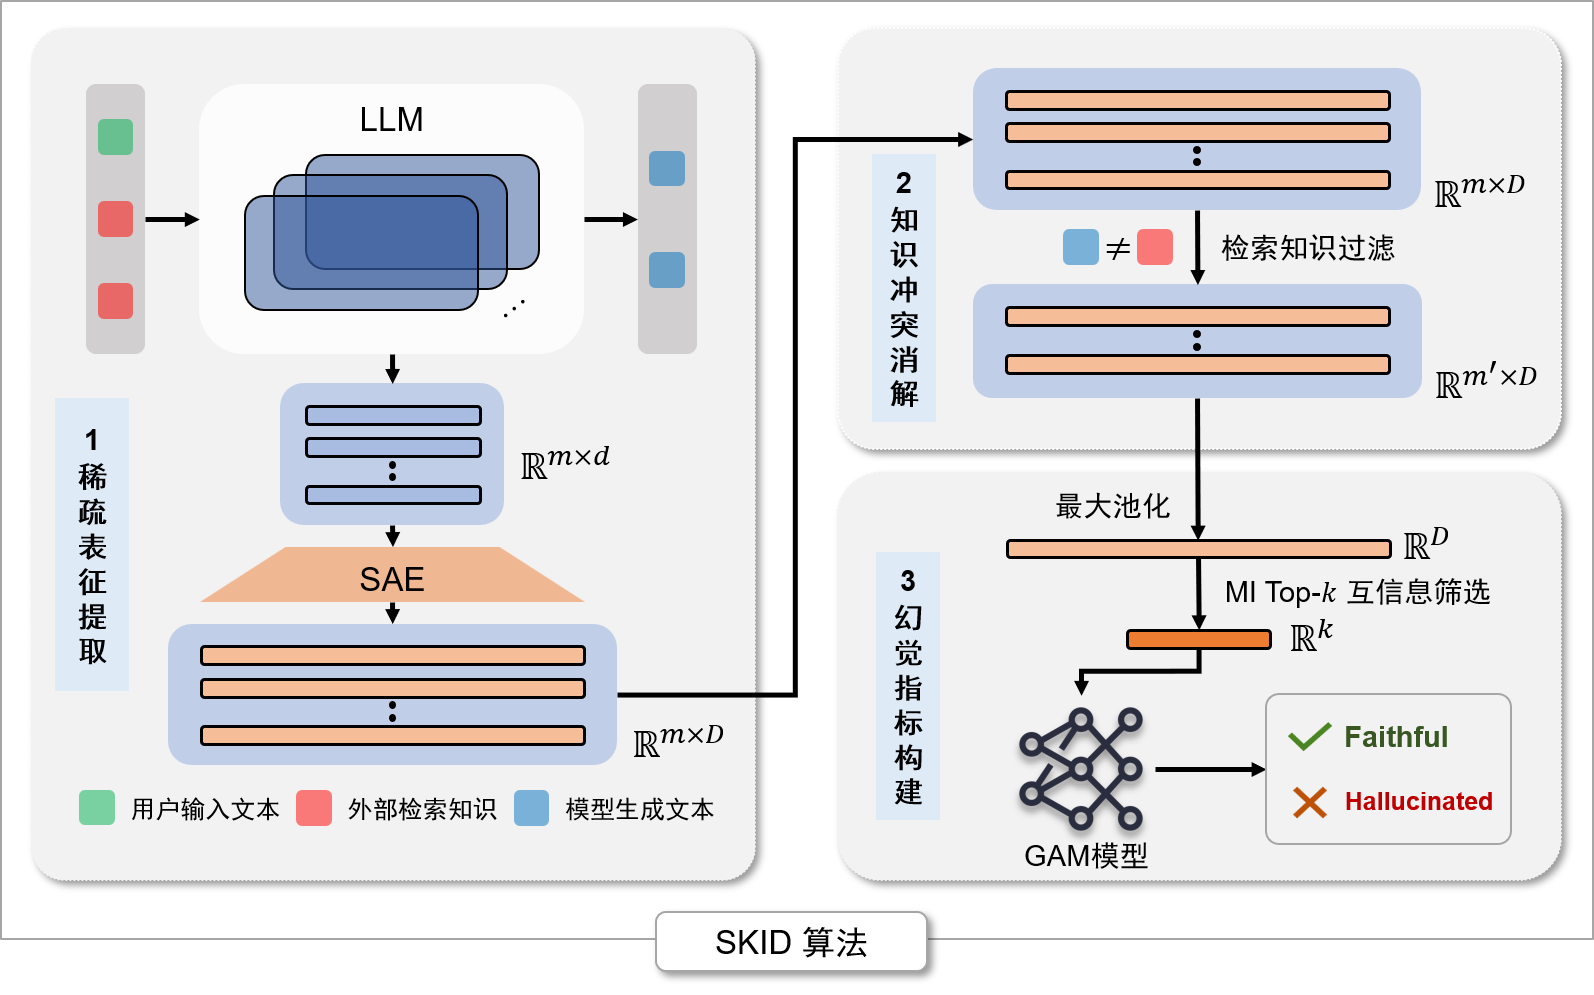
\includegraphics[width=\textwidth]{figures/content/第四章方法总览.png}
    \caption{SKID算法框架图}\label{fig:skid_overview}
\end{figure}

% TODO：画图
% TODO：写算法

\subsection{稀疏表征提取}\label{subsec:sparse_feature_extraction}

% 从大模型生成过程的某层提取output token的表征，通过稀疏自编码器SAE转为高维稀疏表征。
% 高维稀疏表征有什么用，为什么要做这一步。

为刻画大语言模型在生成过程中的内部知识表征，本文首先在模型生成输出序列时提取输出token的中间层隐藏表示，并进一步借助稀疏自编码器将其映射到高维稀疏特征空间中。具体而言，设大语言模型为$M$，对于输入样本，模型生成输出序列$Y=\{y_1,y_2,\dots,y_m\}$。记第$l$层对第$i$个输出token $y_i$的隐藏表示为$\mathbf{h}_i^{(l)}\in\mathbb{R}^{d}$，其中$d$为原始隐空间维度。对于每个输出token，本文选取指定层的隐藏表示作为其内部语义状态的表征，并将其输入预训练好的SAE编码器，得到对应的高维稀疏表征$\mathbf{z}_i=f_{\mathrm{SAE}}\!\left(\mathbf{h}_i^{(l)}\right)\in\mathbb{R}^{D}$，其中$D$为SAE的特征维度，满足$D\gg d$，且$\mathbf{z}_i$具有显著稀疏性，即仅有少量维度被激活。对整个输出序列进行处理后，可得到该样本对应的稀疏特征矩阵
\begin{equation}
\mathbf{Z}=\left [\mathbf{z}_1, \mathbf{z}_2, \cdots, \mathbf{z}_m\right ]^{\top}
\in\mathbb{R}^{m\times D},
\end{equation}
其中第$i$行对应第$i$个输出token的稀疏语义特征表示。

引入高维稀疏表征的核心目的，在于将原始隐藏状态中高度纠缠的语义信息解耦为更具可解释性的特征单元。原始隐表示通常呈现明显的多义性与混合性，即单个神经元或局部子空间往往同时承载多种语义因素，难以直接对应某一明确知识概念；而SAE通过过完备表示与稀疏约束，能够将这种“多义”表征转化为更接近“单义”的稀疏特征激活，使不同维度更倾向于响应相对独立、可解释的语义模式\cite{shu2025survey,bricken2023towards,huben2024sparse,xiong2025toward}。从方法设计上看，这样的特征表示有两方面优势：其一是便于后续对特征空间的互信息筛选和广义加性模型训练，因稀疏式特征便于机器学习建模；其二是有助于提升模型可解释性，可通过分析得知高维空间的具体含义，能够建模何种幻觉，实现从“判定幻觉”到“解释为何被判定为幻觉”的体验提升。

\subsection{知识冲突消解}\label{subsec:knowledge_conflict_resolution}

% 在token级别检索output中在retrieved content中出现过的token，删去这些token，仅保留在output中但未在retrieved content中出现过的token。然后在token维度作max操作，得到batch\_size乘sae\_dim数据。 为什么要删除在检索数据中出现过的token？消解知识冲突，output中包含的外部知识简单去除，留下内部知识信号（幻觉信号）

在获得输出序列的稀疏特征表示之后，本文进一步考虑如何从中分离出更能反映模型内部知识偏差的判别信号。对于RAG任务而言，模型最终生成的输出通常同时混合了两类知识来源：一类是由外部检索文档直接提供或显式支持的知识，另一类则是模型依赖其参数内部所存储知识进行补全、推断甚至臆造时所引入的知识。基于此，本文设计知识冲突消解步骤，在token级别对输出内容进行筛选，以尽可能除去受外部检索知识直接支撑的生成成分，仅保留更可能体现模型内部知识主导作用的部分。

具体而言，设模型输出序列为$Y=\{y_1,y_2,\dots,y_m\}$，检索到的外部知识文本拼接后构成检索内容序列$R=\{D_1, D_2, \dots, D_N\}=\{r_1,r_2,\dots,r_n\}$，其中$D$为文档片段级序列，$r$为token级序列。本文首先在token级别判断输出token是否在检索内容中出现。对于第$i$个输出token $y_i$，定义其对应的指示变量为
\begin{equation}
\delta_i=
\begin{cases}
0, & y_i\in R,\\
1, & y_i\notin R,
\end{cases}
\end{equation}
其中$\delta_i=0$表示该token已经在检索内容中出现，可视为受到外部知识的直接支持；$\delta_i=1$表示该token未在检索内容中出现，更可能反映模型在生成过程中调用内部参数知识后产生的补充或偏移。基于该指示变量，本文对前述token级稀疏表征$\mathbf{z}_i\in\mathbb{R}^{D}$进行筛选，仅保留未在检索内容中出现的输出token所对应的特征，即过滤后的稀疏表征
\begin{equation}
\widetilde{\mathbf{Z}}=\mathbf{Z}\left[\mathbb{I}\left(\delta_i=1\right),:\right]\in\mathbb{R}^{m^\prime\times D},\quad i=1,2,\dots,m.
\end{equation}
其中$\mathbb{I}(\cdot)$为指示函数，表示对$\delta_i=1$的行予以保留，对于$\delta_i=0$的行予以舍弃。于是，对于单个样本，可得到经过知识冲突消解后的token级特征集合$\{\tilde{\mathbf{z}}_1,\dots,\tilde{\mathbf{z}}_{m^\prime}\}$。

在此基础上，为进一步从token级表示汇聚为样本级判别向量，本文沿token维度对过滤后的稀疏特征执行最大池化操作，从而提取每个稀疏维度在当前样本中最显著的激活强度。设单个样本过滤后的稀疏特征矩阵为$\widetilde{\mathbf{Z}}\in\mathbb{R}^{m^\prime\times D}$，则其对应的样本级冲突表征向量定义为
\begin{equation}
\mathbf{s}=\max_{1\leq i\leq m^\prime}\tilde{\mathbf{z}}_i\in\mathbb{R}^{D},
\end{equation}
其中max操作逐维进行，即$s_j=\max_{1\leq i\leq m^\prime}\tilde{z}_{i,j},\quad j=1,2,\dots,D$。

之所以在token维度采用逐维最大池化，而非均值池化或求和聚合，是因为SAE得到的表征通常经过ReLU等非线性激活后呈现出显著的稀疏性，其大多数维度取值为$0$，而非零正值则表示相应语义特征在当前token处被激活。对于同一输出序列而言，某一稀疏特征是否在任意位置被显著触发，往往比其在所有token上的平均响应强度更具有判别意义。逐维最大池化能够有效保留每个特征在样本范围内最强的激活信号，避免池化操作被稀释，从而更有利于后续模型捕捉与幻觉相关的关键知识冲突模式。

之所以滤除在检索数据中已经出现过的输出token，核心原因在于这些token所对应的高维稀疏表征信息在很大程度上已经由外部检索知识显式提供，其激活更可能反映模型对检索内容的复述、复制或局部重组，而非模型对内部知识的利用。若将这些成分保留在检测特征中，则模型可能更多学习到“哪些内容被检索文档支持”，而不是“哪些内容脱离了检索支持却仍被模型生成”，从而弱化对RAG幻觉本质的刻画。相较之下，那些出现在输出中、却未在检索知识中出现的token，更有可能承载模型内部知识外溢、过度推断或错误补全所形成的幻觉信号。因此，通过在token级别去除被外部知识直接覆盖的生成成分，本文实现了对内外知识混合信号的初步解耦，将检测重点集中于更具判别价值的内部知识残差信号之上。

从方法机理上看，这一过程即为一种面向RAG场景的知识冲突消解操作。经过检索增强后，模型输出中的一部分内容与外部知识是一致的、受支持的，这部分内容本身应当并不构成幻觉；真正需要关注的是那些未被检索证据覆盖、但仍在输出中被激活和表达出来的内容，因为它们更可能来源于模型内部参数知识，并在外部证据约束不足或内外知识不一致时表现为事实性偏差。本文通过简单而直接的token滤除策略，在token层级将输出中包含的外部知识成分尽可能去除，从而保留下更纯净的内部知识信号，也即更接近幻觉本质的检测信号。这样的设计不仅与RAG场景下“外部知识约束生成”的任务设定更加一致，也更加契合RAG场景下幻觉检测的任务特点，为后续基于稀疏特征维度分析模型为何产生幻觉提供了更加清晰的表示基础。

\subsection{幻觉指标构建}\label{subsec:skid_hallucination_score_definition}

% 对batch\_size乘sae\_dim维数据每维度和已有的幻觉0/1标签计算互信息。取互信息最高的k个维度。得到batch\_size乘k的矩阵。对这矩阵训练简单GAM（EBM）分类器拟合。测试时遵循同样的步骤。 现在写这个部分。注意简单介绍一下GAM和互信息的作用，但不要太长，重点放在我的方法本身。

在完成知识冲突消解后，本文已经为每个样本获得了样本级稀疏冲突表征$\mathbf{s}\in\mathbb{R}^{D}$。然而，并非所有稀疏特征维度都与RAG幻觉判别具有同等关联：部分维度可能主要反映一般性的语言模式或无关语义因素，另一些维度则更可能直接刻画模型内部知识与外部检索知识之间的冲突强度。因此，本文进一步在特征维度上进行判别性筛选，从中选取与幻觉标签最相关的关键稀疏特征，并基于这些特征构建最终的幻觉检测指标。

具体而言，设训练集共有$N$个样本，经过前述步骤后可得到样本级特征矩阵$\mathbf{S}_{\mathrm{train}}\in\mathbb{R}^{N\times D}$，其中第$i$个样本的幻觉标签记为$c_i\in\{0,1\}$，$c_i=1$表示该样本存在幻觉，$c_i=0$表示该样本不存在幻觉。对于第$j$个稀疏特征维度，记其在全部训练样本上的取值为随机变量$S_j$，对应的标签随机变量记为$C$，则本文计算该维度与幻觉标签之间的互信息
\begin{equation}
I(S_j;C),\quad j=1,2,\dots,D.
\end{equation}

互信息可用于度量某一特征维度与标签变量之间的统计相关程度。与仅刻画线性相关性的指标相比，互信息能够更一般地反映特征对标签判别所提供的信息量，因此适合作为高维稀疏特征筛选的依据。基于此，本文按照$I(S_j;C)$从高到低对全部$D$个特征维度进行排序，并选取其中互信息最高的$k$个维度构成关键特征集合
\begin{equation}
\mathcal{K}=\{j_1,j_2,\dots,j_k\},\quad |\mathcal{K}|=k.
\end{equation}
据此，可从原始特征矩阵$\mathbf{S}_{\mathrm{train}}$中抽取对应的低维判别特征，得到
\begin{equation}
\mathbf{F}_{\mathrm{train}}=\mathbf{S}_{\mathrm{train}}[:,\mathcal{K}]\in\mathbb{R}^{N\times k}.
\end{equation}

上述过程的核心作用，在于从高维稀疏冲突表征中进一步提炼出与幻觉最相关的少量特征维度。一方面，SAE诱导的特征空间通常具有较高维数，若直接使用全部维度进行建模，容易引入冗余信息与噪声信号，削弱检测器对关键冲突模式的敏感性；另一方面，互信息筛选能够保留那些对幻觉判别最具信息贡献的稀疏维度，使最终检测指标更加集中地反映“哪些内部知识特征的激活与幻觉出现最为相关”。因此，这一步不仅实现了特征降维，也进一步增强了检测信号的判别性与可解释性。

在获得$\mathbf{F}_{\mathrm{train}}$之后，本文采用广义加性模型（Generalized Additive Model，GAM）作为最终的幻觉检测器，对幻觉标签进行拟合。GAM的基本思想是将模型输出表示为若干单变量或低阶交互项的可加和，从而在保持一定非线性拟合能力的同时，维持较好的可解释性。对于本文任务，设输入样本的$k$维特征向量为$\mathbf{f}=(f_1,f_2,\dots,f_k)$，则分类器的判别函数可表示为
\begin{equation}
g(\mathbf{f})=\beta_0+\sum_{t=1}^{k}\alpha_t(f_t),
\end{equation}
其中$\beta_0$为偏置项，$\alpha_t(\cdot)$表示第$t$个特征维度对应的单变量响应函数。在二分类设置下，模型输出样本存在幻觉的概率为
\begin{equation}
P\left(C=1|\mathbf{f}\right)=\sigma\!\left(g(\mathbf{f})\right),
\end{equation}
其中$\sigma(\cdot)$表示Sigmoid函数。

本文选择简单GAM而非更复杂的黑盒分类器，主要出于轻量化需要考虑。作为需要训练的模型，经过前述知识冲突消解与互信息筛选后，输入特征已经被压缩为一组参数量较少且具有明确判别意义的关键稀疏维度，此时使用结构简单的可加模型即可较好地拟合幻觉与特征之间的关系，无需额外引入过强的模型复杂度。

综上，本文结合SAE稀疏特征和内外知识冲突消解，构建面向RAG幻觉检测的最终指标，其生成流程如下：首先在训练集上取大模型某层输出隐藏表征，通过SAE模型升维为高维稀疏特征。随后，从输出中筛去在检索知识中出现过的token，以消解知识冲突。其次，计算每个SAE特征维度与幻觉标签之间的互信息，选取最具判别力的$k$个关键维度。最后以这些关键维度构成的$N\times k$特征矩阵为输入，训练GAM分类器拟合幻觉标签，从而得到从稀疏冲突特征到幻觉概率的映射关系。此流程中，数据结构经各种函数操作变换，式~\ref{eq:data_shape}清晰地展示了数据形状的变化。
\begin{equation}
  \label{eq:data_shape}
  \mathbf{h}^{(l)}\in\mathbb{R}^{m\times d} \xrightarrow[\text{编码}] {\text{SAE}}
  \mathbf{Z}\in\mathbb{R}^{m\times D} \xrightarrow[\text{冲突消解}]{\text{检索知识}} 
  \widetilde{\mathbf{Z}}\in\mathbb{R}^{m^\prime\times D} \xrightarrow[\text{最大池化}]{\text{token}} 
  \mathbf{s}\in\mathbb{R}^{D} \xrightarrow[\text{特征筛选}]{\text{互信息}} 
  \mathbf{f}\in\mathbb{R}^{k} \xrightarrow{\text{GAM}} 
  \mathbb{R}.
\end{equation}

对于测试阶段，本方法遵循与训练阶段完全一致的处理流程：首先从模型输出中提取稀疏表征，并经由知识冲突消解得到样本级特征向量；然后仅保留训练阶段确定的关键维度集合$\mathcal{K}$，构造测试特征矩阵$\mathbf{F}_{\mathrm{test}}\in\mathbb{R}^{N_{\mathrm{test}}\times k}$；最后将其输入训练阶段得到的GAM分类器，输出对应样本的幻觉预测结果与幻觉概率分数。由此，本文完成了从高维稀疏知识冲突表征到最终RAG幻觉检测指标的构建。上述SKID算法的步骤清晰地总结于算法~\ref{alg:skid_train}及算法~\ref{alg:skid_test}中。

\begin{algorithm}[htbp]
\caption{SKID算法（训练阶段）}
\label{alg:skid_train}
\begin{algorithmic}[1]
\Require 训练集$\mathcal{D}_{\mathrm{train}}=\{(X^{(u)},R^{(u)},Y^{(u)},c^{(u)})\}_{u=1}^{N}$；大语言模型$M$；指定层索引$l$；稀疏自编码器$f_{\mathrm{SAE}}(\cdot)$；保留特征维数$k$
\Ensure 关键特征集合$\mathcal{K}$；训练好的GAM分类器$\mathcal{G}$

\For{$u=1,2,\dots,N$}
    \State 提取样本$(X^{(u)},R^{(u)},Y^{(u)})$中输出序列$Y^{(u)}=\{y^{(u)}_1,\dots,y^{(u)}_{m_u}\}$在第$l$层的隐藏状态$\mathbf{h}^{(l,u)}_i$
    \State $\mathbf{z}^{(u)}_i \gets f_{\mathrm{SAE}}(\mathbf{h}^{(l,u)}_i),\quad i=1,2,\dots,m_u$
    \State 构造稀疏特征矩阵$\mathbf{Z}^{(u)}=[(\mathbf{z}^{(u)}_1)^\top;(\mathbf{z}^{(u)}_2)^\top;\dots;(\mathbf{z}^{(u)}_{m_u})^\top]\in\mathbb{R}^{m_u\times D}$
    \State 依据$y^{(u)}_i\notin R^{(u)}$保留未被检索内容覆盖的输出token，得到过滤后的稀疏特征矩阵$\widetilde{\mathbf{Z}}^{(u)}\in\mathbb{R}^{m'_u\times D}$
    \State 逐维最大池化：$\mathbf{s}^{(u)}\gets \max_{1\leq i\leq m'_u}\widetilde{\mathbf{z}}^{(u)}_i\in\mathbb{R}^{D}$
\EndFor

\State 构造训练特征矩阵$\mathbf{S}_{\mathrm{train}}=[(\mathbf{s}^{(1)})^\top;(\mathbf{s}^{(2)})^\top;\dots;(\mathbf{s}^{(N)})^\top]\in\mathbb{R}^{N\times D}$

\For{$j=1,2,\dots,D$}
    \State 计算第$j$维特征与幻觉标签之间的互信息$I(S_j;C)$
\EndFor

\State 选取互信息最高的前$k$个维度，构成关键特征集合$\mathcal{K}=\{j_1,j_2,\dots,j_k\}$
\State 得到降维后的训练特征矩阵$\mathbf{F}_{\mathrm{train}}=\mathbf{S}_{\mathrm{train}}\left [:, \mathcal{K}\right ]\in\mathbb{R}^{N\times k}$
\State 用$\mathbf{F}_{\mathrm{train}}$及标签$\{c^{(u)}\}_{u=1}^{N}$训练GAM分类器$\mathcal{G}$

\State \Return $\mathcal{K},\mathcal{G}$
\end{algorithmic}
\end{algorithm}

\begin{algorithm}[htbp]
\caption{SKID算法（测试阶段）}
\label{alg:skid_test}
\begin{algorithmic}[1]
\Require 测试样本$(X,R,Y)$；大语言模型$M$；指定层索引$l$；稀疏自编码器$f_{\mathrm{SAE}}(\cdot)$；关键特征集合$\mathcal{K}$；训练好的GAM分类器$\mathcal{G}$
\Ensure 幻觉预测标签$\hat{c}\in\{0,1\}$

\State 提取输出序列$Y=\{y_1,y_2,\dots,y_m\}$在第$l$层的隐藏状态$\mathbf{h}^{(l)}_i$
\State $\mathbf{z}_i \gets f_{\mathrm{SAE}}(\mathbf{h}^{(l)}_i),\quad i=1,2,\dots,m$
\State 构造稀疏特征矩阵$\mathbf{Z}=[\mathbf{z}_1^\top;\mathbf{z}_2^\top;\dots;\mathbf{z}_m^\top]\in\mathbb{R}^{m\times D}$
\State 依据$y_i\notin R$保留未被检索内容覆盖的输出token，得到过滤后的稀疏特征矩阵$\widetilde{\mathbf{Z}}\in\mathbb{R}^{m'\times D}$
\State 逐维最大池化：$\mathbf{s}\gets \max_{1\leq i\leq m'}\widetilde{\mathbf{z}}_i\in\mathbb{R}^{D}$
\State 按关键特征集合$\mathcal{K}$抽取判别特征，得到$\mathbf{f}=\mathbf{s}\left[\mathcal{K}\right]\in\mathbb{R}^{k}$
\State $\hat{c}\gets \mathcal{G}(\mathbf{f})$

\State \Return $\hat{c}$
\end{algorithmic}
\end{algorithm}

\section{实验分析}

本节将通过一系列实验来验证SKID算法在RAG幻觉检测任务中的有效性与泛化能力，并通过消融实验分析不同参数选择、变体构造对检测性能的影响。具体而言，本节将首先介绍实验设置，包括数据集、评测指标和对比方法；随后展示主要实验结果，并与现有主流方法进行对比分析；最后通过消融实验探讨超参数、数据集变体、SAE模块等设计因素对检测性能的影响。

\subsection{实验设置}\label{subsec:skid_experiment_settings}

本文在多个常用RAG幻觉检测数据集上与现有主流方法进行对比评测，以验证SKID算法在不同任务和不同领域上的有效性与泛化能力。参考现有主流工作\cite{xiong2025toward}，在实验中，本文采用四个公开数据集，涵盖了数学问题、常识问答、定理证明、事实性问答等多种任务类型和领域背景；采用幻觉检测领域最常见的三个评价指标来衡量比较算法性能；并与多种当前的主流方法进行性能对比。

\subsubsection{数据集}

% 四个数据集。其中一个有三个子集。

\emph{RAGTruth}\cite{niu2024ragtruth}。RAGTruth是近年来RAG幻觉检测领域中具有代表性的数据集之一，专门面向检索增强生成场景下的幻觉分析与检测任务构建。该数据包含近18,000条在标准RAG流程下由多种大语言模型自然生成的响应样本，并提供了人工标注的幻觉信息。每条数据包含输入、输出及“是否幻觉”的标签。该数据集分为以下三个子集：

\begin{itemize}
  \item \emph{Data2txt}：该子集任务为将社区商户点评类JSON格式数据转为文字总结。
  \item \emph{QA}：该子集任务为根据提供的短文回答阅读理解问题，覆盖百科、常识问题。
  \item \emph{Summary}：该子集任务为根据检索到的新闻文本生成摘要。
\end{itemize}

\emph{Dolly}（Accurate Context）\cite{hu2024refchecker,DatabricksBlog2023DollyV2}。该数据集为RefCheck\cite{hu2024refchecker}基于开源大规模LLM数据集Dolly\cite{DatabricksBlog2023DollyV2}构建，同样包含检索文本的输入及来自大模型的输出，以及幻觉标签，适用于RAG幻觉检测任务。该数据集以开放域事实性问答为主，领域涵盖广泛，如地理、历史、政治、体育等。该数据集没有原生定义的训练与测试集；在实验中将参考已有方法的做法，将其随机平均分为两份以供训练及测试。

除上述数据集外，以下两个数据集也将在~\ref{subsec:skid_ablation}消融实验中使用到，以更全面地体现SKID算法的泛化性能：

\emph{AggreFact}\cite{tang2023understanding}。专为总结型任务中的事实一致性错误收集的数据集，同样包含检索文本的输入及来自大模型的输出，以及幻觉标签，适用于RAG幻觉检测任务。该数据集输出为对新闻文本的事实性总结。

\emph{TofuEval}\cite{tang2024tofueval}。与上述数据集不同，TofuEval专门用于聚焦评估大模型在主题对话摘要任务中的事实一致性。输入数据中包含多说话人的会议对话（标注有说话人信息，场景多为议会辩论），大模型生成的对话总结及幻觉标签。

以上数据集的相关信息总结如表~\ref{tab:skid_datasets}所示。

\begin{table}[htbp]
  \centering
  \caption{SKID实验数据集概览}
  \label{tab:skid_datasets}
  \begin{autofittabular}{lllcc}
  \toprule
  数据集 & 任务类型 & 领域背景 & 样本数（训练/测试） & 幻觉率\%（训练/测试） \\
  \midrule
  RAGTruth & & & 15,090/2700 & 44.54/34.93 \\
  \quad -- Data2txt & JSON转文本 & 社区商户点评 & 5,298/900 & 69.37/64.33 \\
  \quad -- QA & 阅读理解 & 百科常识 & 5,034/900 & 31.07/17.78 \\
  \quad -- Summary & 文本摘要 & 新闻 & 4,758/900 & 31.15/22.67 \\
  Dolly & 阅读理解 & 开放事实问答 & 148/149 & 50.68/52.35 \\
  AggreFact & 文本摘要 & 新闻 & 1,236/1,117 & 35.76/29.54 \\
  TofuEval & 文本摘要 & 会议对话 & 617/267 & 34.20/36.70 \\
  \bottomrule
  \end{autofittabular}
\end{table}

\subsubsection{评价指标}

为全面评估所提方法在RAG幻觉检测任务中的性能表现，本文在主实验中采用与参考工作一致的三个评价指标，即AUROC、ACC和F1。同时，为进一步考察模型在多种阈值设定下的性能，本文额外引入FPR95和AUPR作为补充评价指标。其中，AUROC、FPR95和AUPR已在~\ref{subsec:experiment_settings}中进行介绍，在本章节中沿用相同定义进行评估。

对于准确率（accuracy，ACC），其用于衡量分类器在全部测试样本上的整体判别正确比例。在本实验中，用于判别正负例的阈值设定为0.5，即最终的GAM模型输出高于0.5记为1（幻觉回答样本），否则记为0（忠实回答样本）。设测试集中共有$N$个样本，其中真正例（true positive）、真负例（true negative）、假正例（false positive）和假负例（false negative）的数量分别记为$\mathrm{TP}$、$\mathrm{TN}$、$\mathrm{FP}$和$\mathrm{FN}$，则ACC定义为
\begin{equation}
\mathrm{ACC}=\frac{\mathrm{TP}+\mathrm{TN}}{\mathrm{TP}+\mathrm{TN}+\mathrm{FP}+\mathrm{FN}}.
\end{equation}

该指标能够直接反映模型整体分类结果的正确程度，但在类别分布不均衡时，可能不足以充分体现模型对少数类样本的识别能力。对于F1值，其综合考虑了分类器的精确率（precision）与召回率（recall），能够更平衡地评价模型对正类样本的检测效果。首先，精确率与召回率分别定义为
\begin{equation}
\mathrm{Precision}=\frac{\mathrm{TP}}{\mathrm{TP}+\mathrm{FP}},
\quad \mathrm{Recall}=\frac{\mathrm{TP}}{\mathrm{TP}+\mathrm{FN}}.
\end{equation}
在此基础上，F1值定义为Precision与Recall的调和平均，即
\begin{equation}
\mathrm{F1}=\frac{2\cdot \mathrm{Precision}\cdot \mathrm{Recall}}{\mathrm{Precision}+\mathrm{Recall}}.
\end{equation}
相较于仅考察某一单独指标，F1能够更有效地反映分类器在“减少误报”与“避免漏检”之间的综合表现，因此也是二分类检测任务中常用的重要评价指标。

综上，本文采用AUROC、ACC、F1、FPR95和AUPR五项指标对各方法进行系统评估。其中，AUROC、FPR95和AUPR主要用于衡量模型在不同判别阈值下的整体检测能力与排序能力；ACC和F1则在固定阈值分类决策下，分别从总体正确率与正类识别效果两个角度补充评价模型性能。与~\ref{subsec:experiment_settings}相同，本实验以AUROC为主指标。通过结合多种指标，能够更全面地分析不同方法在RAG幻觉检测任务中的实际表现。

\subsubsection{模型配置}

与\ref{chp:chapter3}中的幻觉检测数据集不同，本方法中使用的针对RAG幻觉检测的数据集均预置“输出”部分，而不依赖特定大模型实时输出。因此，在检测过程中，大模型仅用于编码“输入-输出”文本，用于提取内部表征，并不实际进行数据集所示任务输出。

本实验为便于对比，采用与参考方法一致的Llama-2-7B\footnote{https://huggingface.co/meta-llama/Llama-2-7b\cite{touvron2023llama2}}模型。该大模型属于当前主流的开源指令微调模型之一，性能及参数量较为合适，在保证了一定语义理解力及编码质量的同时，维持了较低的计算开销。对于使用的SAE模型，本文采取了与大模型相对应的开源预训练SAE\footnote{https://huggingface.co/yuzhaouoe/Llama2-7b-SAE\cite{zhao2025steering}}模型，并采用默认的模型第15层的输出隐藏表征计算稀疏表示。该模型将Llama-2-7B原始的隐藏表征维度从4,096维放大32倍至131,072维。本实验中的所有环节均可在一张NVIDIA RTX A6000（显存48GB）显卡上运行。

\subsubsection{对比方法}

为全面评估本文方法的有效性，本文选取了以下具有代表性的RAG幻觉检测与不确定性估计方法作为对比。

\begin{itemize}
  \item RAG幻觉检测方法，包括ReDeEP\cite{sun2025redeep}、RAGLens\cite{xiong2025toward}。该类方法面向检索增强生成场景进行专门设计，重点关注生成内容与检索证据之间的支持关系及其失配现象，与本文所研究的场景完全一致。
  \item 非RAG场景下的白盒幻觉检测方法，包括ITI\cite{li2023inference}、SAPLMA\cite{azaria2023internal}和EigenScore\cite{chen2024inside}。这类方法虽适配于~\ref{chp:chapter3}所示场景，但也可应用于本章的RAG设定。这类方法通常不显式依赖RAG中的外部检索信息，而是从模型内部表征、隐藏状态或统计几何特征中挖掘可用于判别幻觉的信号。
  \item 基于文本引导的大模型自评估方法，包括P(True)\cite{kadavath2022language}和SelfCheckGPT\cite{manakul2023selfcheckgpt}。前者通过提示模型直接估计其输出内容为真的概率，后者则通过多次采样并比较不同生成结果之间的一致性来判断幻觉风险。SelfCheckGPT是该类方法中的代表性工作。
  \item 黑盒统计特征方法，包括LN-Entropy\cite{malinin2021uncertainty}。该类方法不依赖对模型内部机制的显式干预，而是根据生成分布或输出统计量构造检测指标；其中LN-Entropy是一种具有代表性的基于统计不确定性的黑盒特征，应用token长度作归一化，是黑盒方法中性能较好的方法。
\end{itemize}

总体而言，上述基线方法覆盖了从RAG专用检测、通用内部状态分析，到文本自评估与黑盒统计建模等多种技术路线，因此能够为本文方法的性能评估提供较为充分且具有代表性的参照。

\subsection{结果分析}\label{subsec:skid_result_analysis}

本文SKID及对比方法在RAGTruth与Dolly数据集上的实验结果如表~\ref{tab:skid_main_result}所示，各项评价指标为百分数，其中的最佳结果以\textbf{粗体}展示。

\begin{table}[htbp]
  \centering
  \caption{SKID在RAGTruth与Dolly数据集上的实验结果}
  \label{tab:skid_main_result}
  \begin{autofittabular}{lcccccc}
  \toprule
  \multirow{2}{*}{方法} & \multicolumn{3}{c}{RAGTruth} & \multicolumn{3}{c}{Dolly}\\
   & AUROC~$\uparrow$ & ACC~$\uparrow$ & F1~$\uparrow$ & AUROC~$\uparrow$ & ACC~$\uparrow$ & F1~$\uparrow$\\
  \midrule
  LN-Entropy    & 59.12 & 56.20 & 68.50 & 60.74 & 56.56 & 62.61 \\
  P(True)       & 70.93 & 56.48 & 65.49 & 61.91 & 53.44 & 50.95 \\
  SelfCheckGPT  & --    & 58.44 & 46.42 & --    & 53.00 & 31.88 \\
  EigenScore    & 60.45 & 54.22 & 66,82 & 67.86 & 65.96 & \textbf{72.41} \\
  SAPLMA        & 71.07 & 51.55 & 65.02 & 65.00 & 60.84 & 66.53 \\
  ITI           & 67.14 & 56.67 & 64.96 & 54.94 & 58.00 & 62.81 \\ 
  ReDeEP        & 74.58 & 68.22 & 71.90 & 70.55 & 67.23 & 68.03 \\
  RAGLens       & 82.03 & 71.62 & 72.45 & 72.68 & 69.64 & 69.66 \\
  SKID          & \textbf{82.21} & \textbf{71.68} & \textbf{72.48} & \textbf{76.00} & \textbf{69.70} & 69.71 \\
  \bottomrule
  \end{autofittabular}
\end{table}

% 吹嘘一下性能好，踩一下别的方法的弱点。
% 纵向对比分析，我们的方法比其他方法的性能高。尤其是在主指标AUROC上提高较多。另外两个指标上也差不多或者有一定提高。
% 横向对比分析，我们的方法在不同数据集上表现的都不错。

由表~\ref{tab:skid_main_result}总体来看，所提方法在两个数据集上均取得了具有竞争力甚至最优的性能，验证了其在RAG幻觉检测任务中的有效性。表中数据分析如下：

\begin{itemize}
  \item \emph{性能总体优于对比方法。}从纵向对比角度分析，与现有各类方法相比，SKID在核心指标AUROC上均取得了最优结果，在RAGTruth和Dolly数据集上分别达到82.21\%和76.00\%，相较于当前表现较强的RAG专用方法（如ReDeEP与RAGLens）仍有进一步提升。这表明本文方法在不同判别阈值下均具备更稳定、更准确的排序能力，能够更有效地区分幻觉样本与非幻觉样本。在ACC与F1指标上，SKID同样表现出较强竞争力：在RAGTruth数据集上取得三项指标的全面最优，在Dolly数据集上也基本达到最优水平，与最佳结果差距极小，整体性能保持领先。相比之下，部分白盒幻觉检测方法（如ITI、SAPLMA）以及基于统计特征的方法（如LN-Entropy）整体表现相对较弱，说明仅依赖模型内部信号或黑盒统计特征，难以充分刻画RAG场景下“内外知识冲突”这一关键因素。
  \item \emph{显式建模外部检索知识有利于提升性能。}进一步分析不同类别方法的表现，可以发现RAG幻觉检测方法（如ReDeEP与RAGLens）整体优于白盒与黑盒幻觉检测方法方法，验证了显式建模检索知识的重要性。在此基础上，本文方法通过在稀疏特征空间中进行知识冲突消解建模，相较于RAGLens进一步提升了检测性能，说明在高维可解释表征上进行更精细的特征筛选与冲突建模能够带来额外收益。
  \item \emph{整体稳定性较好。}值得注意的是，EigenScore在Dolly数据集上的F1指标达到72.41\%，表现突出，但其在AUROC与ACC指标上相对不稳定，说明其判别能力在不同阈值或不同数据分布下存在一定波动；而本文方法在多个指标上均保持较为均衡的表现，体现出更好的整体稳定性。
  \item \emph{泛化能力强。}从横向对比角度来看，SKID在两个数据集上均取得一致性的优良表现，说明该方法具有较好的跨数据集泛化能力。无论是在以RAGTruth为代表的多来源多任务数据集，还是在Dolly开放式阅读理解问答的数据分布下，SKID均能够稳定提升AUROC等关键指标，表明其所构建的“稀疏特征+知识冲突消解”框架能够有效捕捉RAG幻觉的本质特征，而不依赖于特定数据集的分布特性。\ref{subsec:skid_ablation}进一步从更多数据集和更多评价指标上验证SKID的这一性能特点。
\end{itemize}

综上所述，实验结果充分表明，本文提出的SKID方法在RAG幻觉检测中相较于现有方法具有更优的检测性能和更稳定的表现，尤其在主指标AUROC上取得了显著提升。同时，其在不同数据集上的一致性优势，也验证了方法设计的合理性与泛化能力。

\subsection{消融实验}\label{subsec:skid_ablation}

本小节将进一步在更多评价指标上衡量SKID算法的性能；对RAGTruth数据集、SKID算法的各种变体，以及SKID方法中的各模块进行详细的消融分析；还将从可解释性分析的角度评价SKID算法额外带来的易用性与用户信任度。

\subsubsection{补充评价指标与额外数据集}

如~\ref{subsec:skid_experiment_settings}中所述，除需在设定阈值下评价分类器性能的ACC、F1评价指标外；还有不依赖特定阈值，通过滑动阈值更全面地评价分类器综合表现的AUROC、FPR95和AUPR评价指标。同时，本文也在额外两个数据集AggreFact和TofuEval上衡量了SKID方法的性能。表~\ref{tab:skid_more_metrics_and_datasets}展示了SKID方法与对比方法在更多评价指标和数据集上的性能。此外，为更直观地分析不同算法在RAG幻觉检测任务中的区分能力，本文额外在两个数据集上，将测试集样本按照参考标签划分为“真实回答”与“幻觉回答”两组，并分别统计各方法在两组样本上的分数分布，如图~\ref{fig:distribution_aggrefact_dolly}所示，绘制方法与~\ref{subsec:result_analysis}中所述保持一致。

\begin{table}[htbp]
  \centering
  \caption{SKID在更多评价指标与数据集上的实验结果}
  \label{tab:skid_more_metrics_and_datasets}
  \begin{autofittabular}{llccccc}
  \toprule
  数据集 & 方法 & AUROC~$\uparrow$ & FPR95~$\downarrow$ & AUPR~$\uparrow$ & ACC~$\uparrow$ & F1~$\uparrow$ \\
  \midrule
  \multirow{2}{*}{RAGTruth} & RAGLens & 82.03 & 66.67 & 68.80 & 71.62 & 72.45 \\
                            & SKID    & \textbf{82.21} & \textbf{63.00} & \textbf{69.41} & \textbf{71.68} & \textbf{72.48} \\
  \midrule
  \multirow{2}{*}{Dolly}    & RAGLens & 72.68 & 80.28 & 73.63 & 69.64 & 69.66 \\
                            & SKID    & \textbf{76.00} & \textbf{63.38} & \textbf{76.60} & \textbf{69.70} & \textbf{69.71} \\
  \midrule
  \multirow{2}{*}{AggreFact}& RAGLens & 80.14 & \textbf{60.10} & 58.18 & 69.45 & 69.33 \\
                            & SKID    & \textbf{82.01}	& 63.41	& \textbf{63.75}	& \textbf{70.33}	& \textbf{71.65} \\
  \midrule
  \multirow{2}{*}{TofuEval} & RAGLens & 73.15	& \textbf{88.17}	& 66.35	& 62.53	& 62.60 \\
                            & SKID    & \textbf{76.09}	& 89.94	& \textbf{68.36}	& \textbf{69.73}	& \textbf{70.50} \\
  \bottomrule
  \end{autofittabular}
\end{table}

\begin{figure}[htbp]
  \centering
  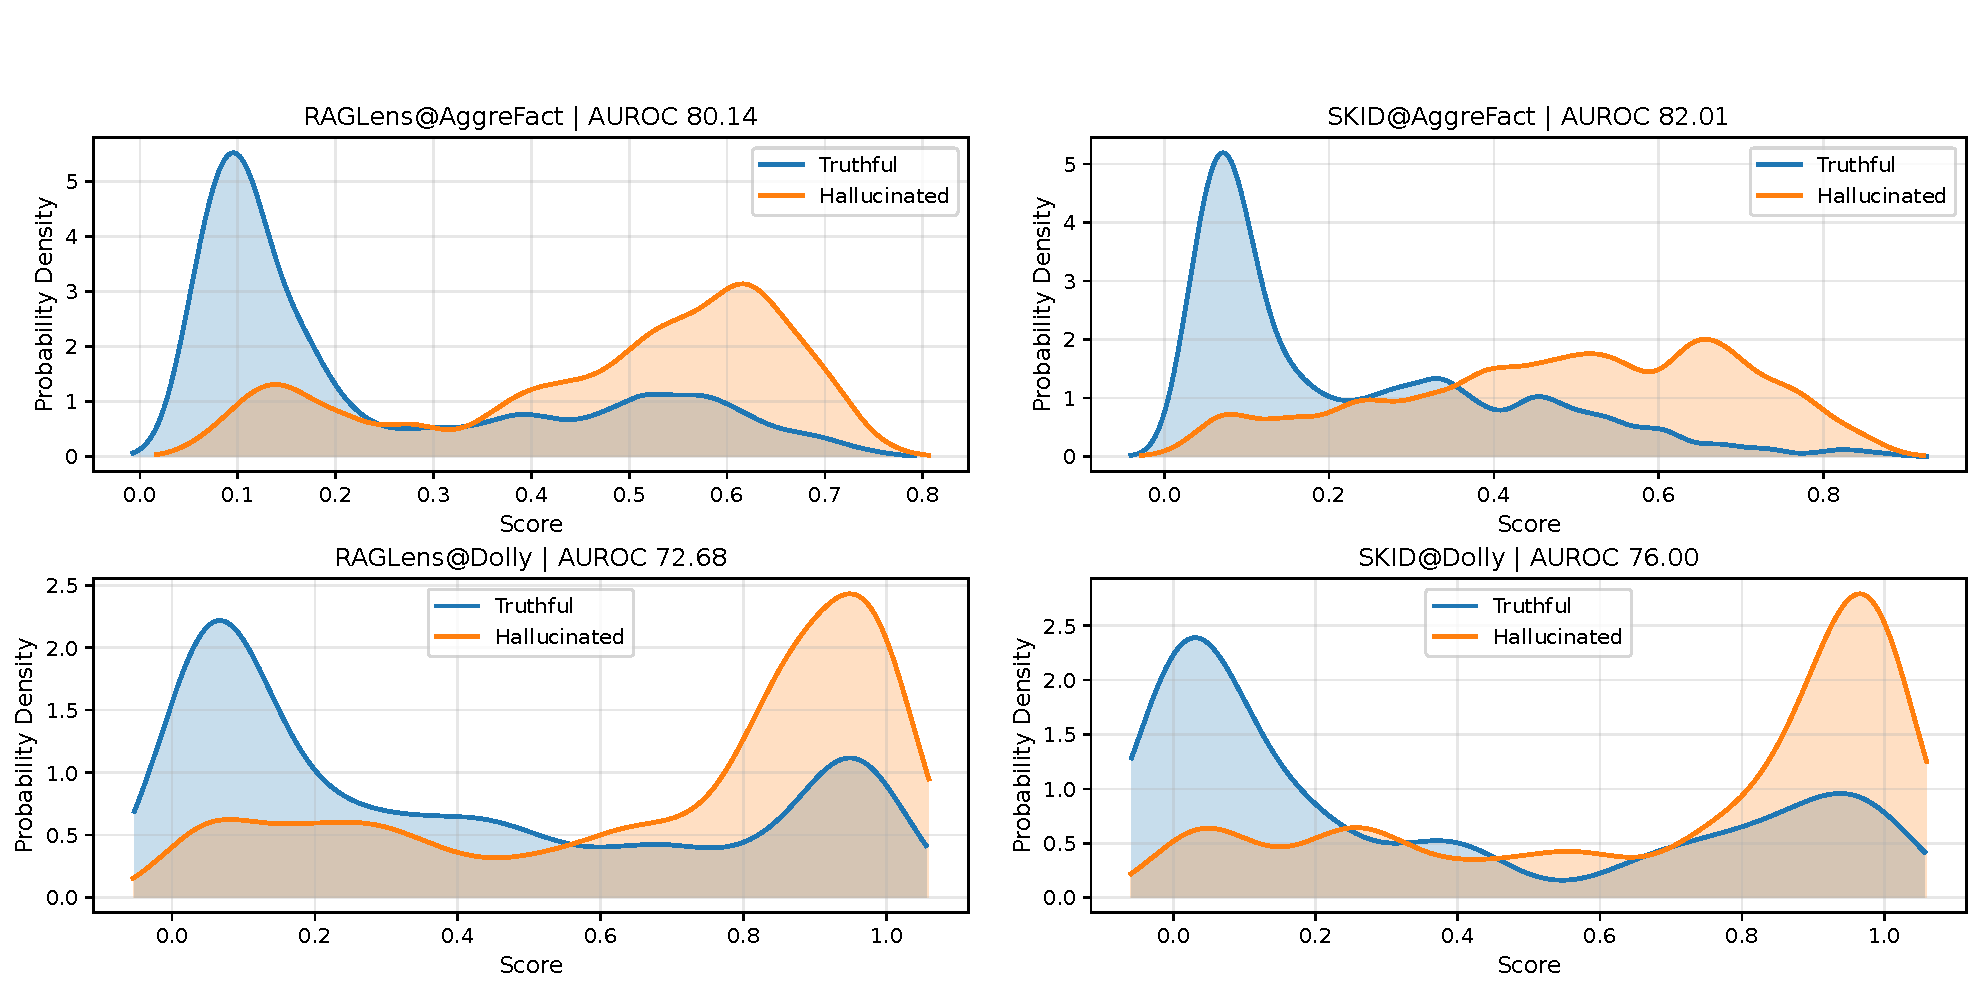
\includegraphics[width=\textwidth]{figures/content/hallucination_score_distribution_2x2_wide.pdf}
  \caption{SKID与RAGLens在AggreFact与Dolly数据集上的幻觉分数分布}
  \label{fig:distribution_aggrefact_dolly}
\end{figure}

从表~\ref{tab:skid_more_metrics_and_datasets}可以看出，在引入更多评价指标与数据集后，SKID方法依然保持了稳定且优越的整体性能。首先，在RAGTruth与Dolly两个数据集上，SKID在AUROC、AUPR以及ACC、F1等多个指标上均优于RAGLens，尤其在FPR95指标上取得了明显下降，表明在保证高召回率的同时，误报率得到了有效控制，从而在阈值无关的检测能力上进一步提升。其次，在额外引入的AggreFact与TofuEval数据集上，SKID同样在大多数指标上取得最优结果，特别是在AUROC与AUPR等综合性指标上表现突出，说明本文方法在不同数据分布与任务设置下均具有良好的泛化能力。尽管在FPR95指标下的个别情况下未取得最优，但整体趋势依然表明SKID在综合性能上优于现有方法。从图~\ref{fig:distribution_aggrefact_dolly}可以看出，在所示数据集上，SKID方法在“真实回答”样本上的分数分布明显偏向于较低的分数区间，而在“幻觉回答”样本上的分数分布则明显偏向于较高的分数区间，显示出较好的区分能力，因此在分类任务中获得了更高的AUROC得分。相比之下，RAGLens方法在两类样本上的分数分布重叠区域较多，占据总数据量的比例较大，说明其在所示数据集上的判别能力相对较弱。综上，实验结果进一步验证了本文方法在多指标、多数据集场景下的稳健性与有效性，亦从可视化的角度验证了SKID在不同数据集上的稳定优越性能，能够更全面地刻画RAG幻觉检测任务中的判别能力。

\subsubsection{数据集变体}

如~\ref{subsec:skid_experiment_settings}中所述，数据集RAGTruth包含三个互不包含的子集，其任务类型、涉及领域各不相同。表~\ref{tab:skid_ragtruth_subsets}展示了SKID方法与对比方法在这三个子集上的具体提升。

\begin{table}[htbp]
  \centering
  \caption{SKID在RAGTruth的三个子数据集上的实验结果}
  \label{tab:skid_ragtruth_subsets}
  \begin{autofittabular}{llccccc}
  \toprule
  数据集 & 方法 & AUROC~$\uparrow$ & FPR95~$\downarrow$ & AUPR~$\uparrow$ & ACC~$\uparrow$ & F1~$\uparrow$ \\
  \midrule
  \multirow{2}{*}{Data2txt} & RAGLens & \textbf{82.03}	& \textbf{69.78}	& \textbf{88.26}	& \textbf{73.64}	& \textbf{74.56} \\
                            & SKID    & 80.62	& 70.40 & 86.04	& 73.33	& 74.37 \\
  \midrule
  \multirow{2}{*}{QA}       & RAGLens & 86.26	& 57.03	& 62.99	& 75.72	& 75.41 \\
                            & SKID    & \textbf{86.49} & \textbf{55.68}	& \textbf{64.88}	& \textbf{75.87}	& \textbf{76.18} \\
  \midrule
  \multirow{2}{*}{Summary}  & RAGLens & 77.55	& 73.42	& 53.29	& 65.04	& \textbf{66.98} \\
                            & SKID    & \textbf{79.46}	& \textbf{62.50}	& \textbf{55.67}	& \textbf{65.41}	& 66.45 \\
  \bottomrule
  \end{autofittabular}
\end{table}

从表~\ref{tab:skid_ragtruth_subsets}可以看出，SKID在不同子任务上的表现存在一定差异。在QA与Summary两个子数据集上，SKID在绝大多数评价指标上均优于RAGLens，特别是在AUROC、FPR95与AUPR等指标上取得稳定提升，表明本文方法在这两类任务中能够更有效地刻画模型内部知识与外部检索知识之间的冲突关系，从而提升幻觉检测性能。相比之下，在Data2txt子数据集上，SKID整体略逊于RAGLens，各项指标均出现一定程度下降。

造成上述差异的一个可能原因在于不同子数据集中检索内容与生成输出的表示形式存在显著差异。在QA与Summary任务中，检索知识与模型输出均以自然语言形式呈现，两者在token层面具有较高的一致性与可对齐性。因此，本文在知识冲突消解步骤中，通过滤除输出中在检索知识中出现过的token，可以较为准确地去除外部知识成分，从而保留更纯净的内部知识信号（即潜在的幻觉信号），使得后续基于稀疏特征的判别更加有效。然而，在Data2txt任务中，虽然最终回答仍以自然语言形式输出，检索知识以结构化的JSON格式给出，其中包含大量非自然语言符号（如花括号、冒号、引号等JSON键值对结构）。除此之外，表格内容表达相对简洁，与最终生成的自然语言输出在表面形式上存在较大差异。在这种情况下，基于token级匹配的筛除策略难以充分覆盖检索知识对应的语义内容，即使某些信息已经在检索知识中出现，其在输出中的自然语言表达形式往往不同，导致这些token无法被有效删除，从而在保留的特征中仍混入较多外部知识信号成分。换言之，知识冲突消解步骤在该子数据集上可能存在“删除不干净”的问题，使得后续构建的检测信号不够纯粹，从而影响整体性能表现。

综上所述，实验结果表明，SKID在自然语言形式一致的RAG场景中能够充分发挥其优势，但在检索内容与生成输出存在显著表达差异（如结构化数据到文本生成）的任务中，其基于token匹配的冲突消解策略仍存在一定局限性。这一现象也为后续工作提供了改进方向，即探索更加语义层面或结构感知的知识对齐与消解方法，以进一步提升方法在复杂RAG场景下的适用性与鲁棒性。

\subsubsection{最高互信息特征筛选维度数$k$}

在~\ref{subsec:skid_hallucination_score_definition}中，本文讨论了幻觉指标构建方法，其中包括从高维稀疏特征中选取其中互信息最高的$k$个维度构成关键特征集合。在本实验中，$k$值的选取与SKID算法的性能存在密切的关系。SKID算法与对比算法在RAGTruth的两个子数据集上的AUROC性能随$k$值变化的趋势如图~\ref{fig:skid_k}所示。

\begin{figure}[htbp]
    \centering
    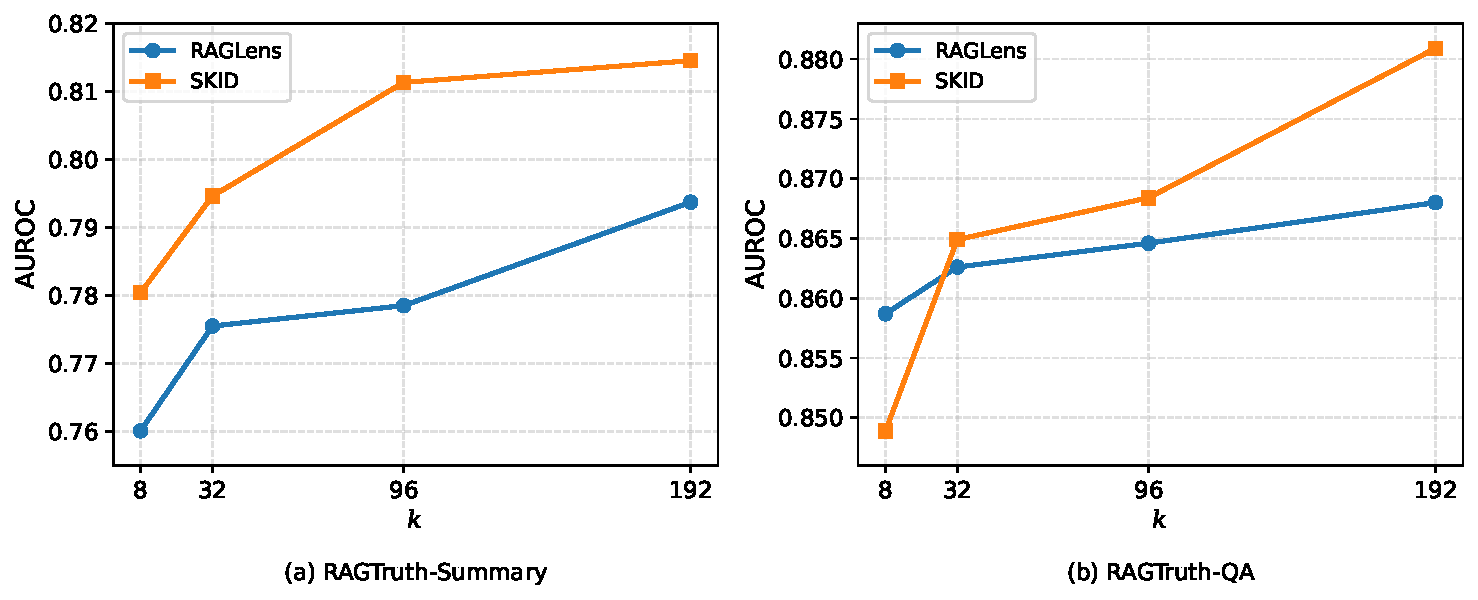
\includegraphics[width=\textwidth]{figures/content/ragtruth_auroc_subplots_v2.pdf}
    \caption{SKID与对比算法在RAGTruth数据集上的AUROC性能随$k$值变化图}\label{fig:skid_k}
\end{figure}

实验结果表明，在不同$k$值设定下，SKID算法在RAGTruth数据集上的性能会随关键特征维度选择而发生明显变化。随着互信息筛选特征维度数$k$的增大，方法在两个数据集上的AUROC整体均呈上升趋势。这一结果与直观感受一致：保留更多高判别性稀疏特征有助于提升RAG幻觉检测性能。过小的$k$值会限制模型对关键知识冲突信号的表征能力，而适当增大$k$能够引入更丰富的判别信息，从而提高检测效果。与此同时，SKID在大多数$k$取值下均优于RAGLens，且这种优势在较大$k$时更加明显，表明所提出的检索知识过滤与稀疏特征建模机制能够更充分地挖掘高维判别特征中的有效信息。总体而言，该实验说明方法对$k$具有一定敏感性，但在合理范围内呈现出较稳定的“随$k$增大而持续受益”的趋势，验证了互信息筛选特征维度在SKID中的重要作用。

\subsubsection{SAE编码模块与知识冲突消解模块}

在~\ref{subsec:sparse_feature_extraction}中，本文讨论了引入高维稀疏表征的核心目的，在于将原始隐藏状态中高度纠缠的语义信息解耦为更具可解释性的特征单元，也便于后续对特征空间的互信息筛选和广义加性模型训练。在~\ref{subsec:knowledge_conflict_resolution}中，本文讨论了知识冲突消解方法的构建，其能显式完成内外知识混合信号的初步解耦，将检测重点集中于更具判别价值的内部知识残差信号之上。表~\ref{tab:skid_module_ablation}直接展示了去除SAE编码模块和知识冲突消解模块前后模型的性能变化。其中，不使用SAE编码模块的实验直接在对应层的$d$维隐藏状态表征（而非经由SAE编码的$D$维高维稀疏表征）上进行后续步骤，如特征筛选、冲突消解、GAM训练等。

\begin{table}[htbp]
  \centering
  \caption{SKID的不同模块变体在TofuEval数据集上的实验结果}
  \label{tab:skid_module_ablation}
  \begin{autofittabular}{ccccccc}
  \toprule
  \multicolumn{2}{c}{模块变体} & \multirow{2}{*}{AUROC~$\uparrow$} & \multirow{2}{*}{FPR95~$\downarrow$} & \multirow{2}{*}{AUPR~$\uparrow$} & \multirow{2}{*}{ACC~$\uparrow$} & \multirow{2}{*}{F1~$\uparrow$} \\
  SAE编码 & 知识冲突消解 & & & & & \\
  \midrule
  $\times$ & $\times$ & 63.12	& 88.67	& 47.86	& 61.07	& 61.33 \\
  $\checkmark$ & $\times$ & 73.15	& 88.17	& 66.35	& 62.53	& 62.60 \\
  $\times$ & $\checkmark$ & 73.93	& \textbf{84.02} & 66.67	& 65.16	& 65.65 \\
  $\checkmark$ & $\checkmark$ & \textbf{76.09} & 89.94	& \textbf{68.36}	& \textbf{69.73}	& \textbf{70.50} \\
  \bottomrule
  \end{autofittabular}
\end{table}

从表~\ref{tab:skid_module_ablation}的结果可以看出，引入SAE编码模块或知识冲突消解模块均能够在不同程度上提升模型的整体检测性能，二者结合时效果最为显著。

具体而言，在不使用任何模块的基线设置下，模型整体表现最弱，说明直接在原始隐藏状态上进行建模难以有效刻画RAG场景下的幻觉信号。当仅引入SAE编码模块时，AUROC与AUPR均有显著提升，表明高维稀疏表征能够有效解耦原始隐状态中的纠缠语义信息，从而为后续判别模型提供更加结构化且可分离的特征空间。当仅引入知识冲突消解模块时，模型同样取得明显提升，说明通过显式去除与检索内容重合的token，可以有效削弱外部知识干扰，使得剩余信号更集中地反映模型内部生成偏差，从而提升幻觉检测的敏感性。

当SAE编码与知识冲突消解同时使用时，模型在大多数指标上取得最优结果，整体性能优于任一单独模块。这表明两者之间具有良好的叠加性：SAE负责提供可解释的稀疏特征空间，而知识冲突消解则进一步净化该空间中的外部知识干扰，从而共同构建出更加稳定且具有判别性的幻觉检测信号。综上，实验结果验证了本文模块设计的合理性，即稀疏表征学习与知识冲突消解对于提升RAG幻觉检测性能均具有关键作用，并且二者的结合能够带来最优的整体效果。

\subsubsection{可解释性}

如~\ref{subsec:skid_hallucination_score_definition}中所述，依据互信息值的大小可以筛选出与幻觉标签相关性最高的$k$个维度。借由SAE的表征能力，这些高维表征空间的具体维度，可能具有一定的单义性和可解释性。如下的实验中，本文在TofuEval数据集中进一步发掘这$k$维数据，借助外置商业大模型强大的文本理解和归纳总结能力，尽可能地探索这些表征幻觉的维度的潜在真实语义。

具体而言，本文设计了一种基于高互信息维度的语义归纳实验流程，以探索SAE表征空间中与幻觉行为相关的潜在语义结构。实验流程如下：

\begin{itemize}
  \item 首先，在通过互信息分析筛选得到的$k$个高相关维度基础上，针对每一个维度，选取该维度激活值最高的$d$个样本。这一步确保了所选样本在该维度上具有最显著的表征响应，有助于增强后续语义分析的信号强度。
  \item 随后，对于每一个高互信息维度，将对应筛选出的$d$个样本回溯至其原始输入与模型输出文本，构建得到$k$组样本集合，每组包含$d$个“高响应”实例。通过这种方式将抽象的神经表征维度映射为具体的文本行为集合，从而建立“表征维度—模型行为”的对应关系。
  \item 在此基础上，在线利用GPT-5.4\footnote{https://openai.com/zh-Hans-CN/index/introducing-gpt-5-4/}——当前性能最强的主流商业大模型之一，作为语义归纳器，对每一组包含$d$个样本的文本集合进行统一分析。具体地，将同一维度下的$d$个输入-输出对作为整体输入提示给大模型，并要求其总结这些回答是否存在共性特征，例如是否倾向于产生事实性错误、是否表现出过度推测、是否存在知识幻觉倾向等。通过这种方式能够从数据驱动的角度，对每个高互信息维度所编码的行为模式进行归纳式解释。
\end{itemize}

上述实验通过对$k$个维度分别获得其对应的语义总结结果，从而构建“维度—幻觉行为描述”的映射表。该映射关系有助于进一步理解SAE中不同稀疏特征在幻觉检测任务中的功能分工，并为后续基于可解释特征的检测方法设计提供依据。实验结果如表~\ref{tab:skid_interpretability}所示。在实验中，本文选取$k=5$，$d=10$进行实验，其他设定与表~\ref{tab:skid_more_metrics_and_datasets}所示的实验设置一致。

\begin{table}[htbp]
  \centering
  \caption{SKID在TofuEval上的可解释性分析}
  \label{tab:skid_interpretability}
  \begin{autofitxtabular}{lllY}
  \toprule
  维度序号 & 互信息 & 幻觉类型 & 具体解释 \\
  \midrule
  119,691 & 0.1095 & 解释性补全 & 将原文里模糊、残缺、未言尽的内容，自动补成完整的因果链、后果链和价值判断 \\
  127,083 & 0.1082 & 细节性补全 & 在原文只提到“申请/讨论/审议”时，补出具体条款、限制条件、实施细节、作用效果 \\
  94,462 & 0.1068 & 具体事实补写 & 将未提及的具体人名、地点、投票结果、身份、条件直接写为确定事实 \\
  10,418 & 0.1002 & 议题混入 & 仍然围绕当前主议题，但混入其他相近政策、法案、提案或背景内容 \\
  79,300 & 0.0983 & 整体议题错配 & 未围绕当前议题，输出几乎全文与输入所讨论议题完全无关 \\
  \bottomrule
  \end{autofitxtabular}
\end{table}

从表~\ref{tab:skid_interpretability}可以看出，基于SAE提取的高互信息稀疏维度并非仅仅对应某种模糊的“低分辨率信号”，而是能够稳定地指向若干具有明确语义边界的幻觉模式，这充分体现了SAE表征在可解释性上的显著优势。具体而言，不同高互信息维度所对应的样本集合并未呈现出杂乱无章的分布，而是分别集中于“解释性补全”“议题混入”以及“整体议题错配”等具有较强一致性的幻觉行为模式。这说明，SAE所学习到的稀疏特征在一定程度上将原本纠缠于隐藏状态中的多种错误模式解耦为相对独立的语义单元。换言之，SKID最终用于判别的并不是难以理解的黑盒分数，而是一组能够被自然语言刻画、并可对应到具体文本行为的稀疏特征，这使得模型具备了较强的事后解释能力。

进一步地，上述结果也从侧面验证了本文设计中引入SAE模块的必要性。若直接在原始稠密隐藏状态上进行分析，不同语义因素往往高度耦合，单个维度通常难以对应稳定而清晰的行为模式；而经过SAE映射后，特征空间中的部分维度能够被赋予更强的单义性，从而使“高响应样本检索—共性行为归纳—幻觉类型命名”这一分析链条成为可能。尤其值得注意的是，这些被识别出的维度不仅能够区分“是否幻觉”，还能够进一步揭示“幻觉是以何种形式发生的”。这意味着SKID的优势不仅体现在检测性能上，还体现在其能够提供更细粒度的错误结构认知，可能为后续的幻觉归因、风险分析以及定向纠正提供了可操作的依据。

总体而言，该实验表明，SAE为SKID带来的并非简单的特征压缩或维度变换，而是一种更具语义可读性的表征重构机制。借助这一机制，模型内部原本难以直接理解的激活模式被转化为具有可命名、可归纳、可分析特性的稀疏特征，从而显著增强方法在实际应用中的易用性和用户信任度。这种“检测性能与语义可解释性并重”的特性，也正是SKID相较于传统黑盒判别方法的重要优势之一。

\section{本章小结}

本章围绕大语言模型RAG幻觉检测问题，在明确任务设定的基础上，提出了基于检索知识冲突消解的SKID方法。该方法首先借由稀疏自编码器将大模型特定层的隐式表征映射到高维系数空间，以将原始隐藏状态中高度纠缠的语义信息解耦为更具可解释性的特征单元；随后筛选滤除输出文本中已于检索知识中出现过的token，以解耦内外知识混合信号，将检测重点集中于更具判别价值的内部知识残差信号之上；最终，从特征维度基于互信息指标筛选出最具幻觉表征能力的少部分特征，训练广义加性分类器，得到最终的幻觉检测信号。

实验结果表明，SKID在多个数据集和多种评价指标上均具有良好的竞争力，整体优于多种类型的基线方法。更多消融实验则进一步证明了SKID算法在更多数据集变体、评价指标上的稳定性能，各模块步骤的设置合理性，以及优越的可解释性。综合来看，本章方法在无需任何额外计算量的情况下提升了RAG幻觉检测的性能，充分利用外部检索知识消解了知识冲突，为后续相关研究提供了坚实的方法基础。
